\documentclass[landscape]{article}
\usepackage{graphicx,amssymb,color}
\pagestyle{empty}
\oddsidemargin  -0.5 in
\evensidemargin -0.5 in
\headheight     0 in
\topmargin      -1 in
\textheight     7.7 in
\textwidth      10 in
\newenvironment{slide:nopage}[1][ ]{\mbox{\bf #1 } \vfill}{\vfill \mbox{ } \pagebreak}
\newenvironment{slide}[1][ ]{\mbox{\bf #1 } \vfill}{\vfill \mbox{ } \hfill \Large \arabic{page} \pagebreak}

\newcommand{\subs}[1]{{\mbox{\large #1}}}
\newcommand{\inv}{$^{-1}$}
\newcommand{\PM}{$\pm$}
\newcommand{\ups}{$\Upsilon$}
\newcommand{\gee}{{\boldmath $\Gamma_{ee}$}}
\newcommand{\us}{$\Upsilon(1S)$}
\newcommand{\uss}{$\Upsilon(2S)$}
\newcommand{\usss}{$\Upsilon(3S)$}
\newcommand{\es}{$\epsilon_{1S}$}
\newcommand{\ess}{$\epsilon_{2S}$}
\newcommand{\esss}{$\epsilon_{3S}$}
\newcommand{\ee}{$e^+e^-$}
\newcommand{\mumu}{$\mu^+\mu^-$}
\newcommand{\tautau}{$\tau^+\tau^-$}
\newcommand{\gamgam}{$\gamma\gamma$}
%\newcommand{\ggg}{$ggg$}
\newcommand{\gggamma}{$gg\gamma$}
\newcommand{\qqbar}{$q\bar{q}$}
\newcommand{\bee}{${\mathcal B}_{ee}$}
\newcommand{\bmm}{${\mathcal B}_{\mu\mu}$}
\newcommand{\btt}{${\mathcal B}_{\tau\tau}$}
\newcommand{\bcas}{${\mathcal B}_\subs{cas}$}
\newcommand{\geehadtot}{$\Gamma_{ee}\Gamma_\subs{had}/\Gamma_\subs{tot}$}
\newcommand{\twotoone}{$\Upsilon(2S) \to \pi^+\pi^- \Upsilon(1S)$}
\newcommand{\pipi}{$\pi^+\pi^-$}
\newcommand{\evis}{$\epsilon_\subs{vis}$}
\newcommand{\ecuts}{$\epsilon_\subs{cuts}$}
\newcommand{\ebeam}{$E_\subs{beam}$}
\newcommand{\ecm}{$E_\subs{CM}$}
\newcommand{\pmax}{$|\vec{p}_\subs{max}|$}
\newcommand{\visen}{$E_\subs{vis}$}
\newcommand{\dxy}{$d_\subs{XY}$}
\newcommand{\dz}{$d_\subs{Z}$}
\newcommand{\vtd}{$V_{td}$}
\newcommand{\twotrack}{{\tt two-track}}
\newcommand{\hadron}{{\tt hadron}}
\newcommand{\radtau}{{\tt rad-tau}}
\newcommand{\eltrack}{{\tt $e^\pm$-track}}
\newcommand{\barrelbhabha}{{\tt barrel-bhabha}}
\newcommand{\axial}{{\tt AXIAL}}
\newcommand{\stereo}{{\tt STEREO}}
\newcommand{\cblo}{{\tt CBLO}}
\newcommand{\cbmd}{{\tt CBMD}}
\newcommand{\cbhi}{{\tt CBHI}}

\begin{document}
\huge \sffamily
\renewcommand{\labelitemi}{{\LARGE $\stackrel{\bullet}{\mbox{ }}$}}
\setlength{\parindent}{0 cm}

\begin{slide:nopage}
\begin{center}
\Huge
  Di-electron Widths of the $\Upsilon$(1S), $\Upsilon$(2S), and $\Upsilon$(3S)

  \vspace{1 cm}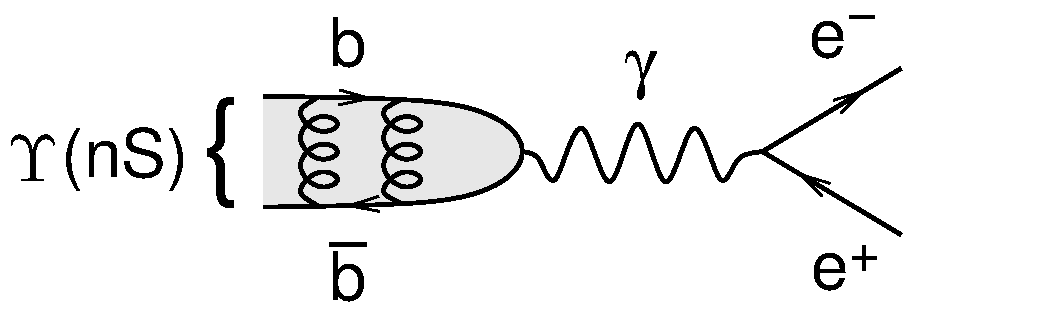
\includegraphics[width=0.5\linewidth]{diagram_GeeU}

  \vspace{2 cm} Jim Pivarski

  \vspace{1 cm} Cornell University

  \vspace{1 cm} CLEO Collaboration
\end{center}
\end{slide:nopage}

\addtocounter{page}{-1}

\begin{slide}[Motivation for a New High-Precision Measurement]

\begin{itemize}\setlength{\itemsep}{1 cm}

  \item Di-electron width \gee\ is a basic parameter of the \ups\ meson

  \item ``Golden-mode'' test of high-precision Lattice QCD

\end{itemize}

\vspace{0.5 cm}
{\color{white} Staggered-quark formalism makes QCD simulations with realistic $u$,
$d$, $s$ masses possible}

\vspace{0.5 cm}
{\color{white} Allows few-percent calculations of observables such as \gee}

\vspace{0.5 cm}
{\color{white} Our high-precision measurement of \gee\ confirms or refutes this calculation}

\vspace{0.75 cm}
\begin{tabular}{p{0.6\linewidth} p{0.4\linewidth}}
  \begin{minipage}{\linewidth}
    \begin{itemize}\setlength{\itemsep}{1 cm}
      \item This test is relevant for CKM element \vtd
    \end{itemize}

    \vspace{0.5 cm}
    {\color{white} $f_B$ is a QCD factor that obfuscates \vtd\ (blue band)}

    \vspace{1 cm}
    {\color{white} \begin{tabular}{r l}
      \gee\ and $f_B$ share: & NRQCD action \\
                             & staggered-quark formalism \\
      but not: & heavy-light quark asymmetry \\
               & axial vector coupling
    \end{tabular}}

  \end{minipage} &
  \begin{minipage}{\linewidth}
    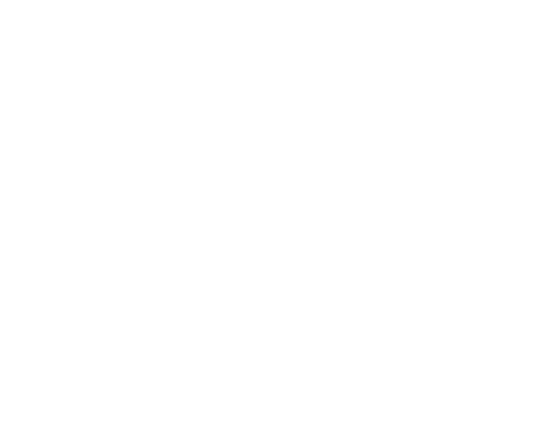
\includegraphics[width=\linewidth]{ckm04-white}
  \end{minipage}
\end{tabular}

\vspace{0.5 cm}
{\color{white} Complementary with $f_D$: see Topher Cawlfield's talk}

\end{slide}

\addtocounter{page}{-1}

\begin{slide}[Motivation for a New High-Precision Measurement]

\begin{itemize}\setlength{\itemsep}{1 cm}

  \item Di-electron width \gee\ is a basic parameter of the \ups\ meson

  \item ``Golden-mode'' test of high-precision Lattice QCD

\end{itemize}

\vspace{0.5 cm}
{\color{black} Staggered-quark formalism makes QCD simulations with realistic $u$,
$d$, $s$ masses possible}

\vspace{0.5 cm}
{\color{black} Allows few-percent calculations of observables such as \gee}

\vspace{0.5 cm}
{\color{blue} High-precision \gee\ measurement tests high-precision \gee\ calculation}

\vspace{0.75 cm}
\begin{tabular}{p{0.6\linewidth} p{0.4\linewidth}}
  \begin{minipage}{\linewidth}
    \begin{itemize}\setlength{\itemsep}{1 cm}
      \item This test is relevant for CKM element \vtd
    \end{itemize}

    \vspace{0.5 cm}
    {\color{white} $f_B$ is a QCD factor that obfuscates \vtd\ (blue band)}

    \vspace{1 cm}
    {\color{white} \begin{tabular}{r l}
      \gee\ and $f_B$ share: & NRQCD action \\
                             & staggered-quark formalism \\
      but not: & heavy-light quark asymmetry \\
               & axial vector coupling
    \end{tabular}}

  \end{minipage} &
  \begin{minipage}{\linewidth}
    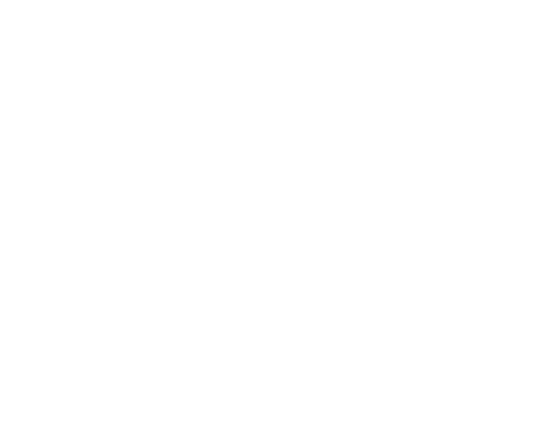
\includegraphics[width=\linewidth]{ckm04-white}
  \end{minipage}
\end{tabular}

\vspace{0.5 cm}
{\color{white} Complementary with $f_D$: see Topher Cawlfield's talk}

\end{slide}

\addtocounter{page}{-1}

\begin{slide}[Motivation for a New High-Precision Measurement]

\begin{itemize}\setlength{\itemsep}{1 cm}

  \item Di-electron width \gee\ is a basic parameter of the \ups\ meson

  \item ``Golden-mode'' test of high-precision Lattice QCD

\end{itemize}

\vspace{0.5 cm}
{\color{black} Staggered-quark formalism makes QCD simulations with realistic $u$,
$d$, $s$ masses possible}

\vspace{0.5 cm}
{\color{black} Allows few-percent calculations of observables such as \gee}

\vspace{0.5 cm}
{\color{blue} High-precision \gee\ measurement tests high-precision \gee\ calculation}

\vspace{0.75 cm}
\begin{tabular}{p{0.6\linewidth} p{0.4\linewidth}}
  \begin{minipage}{\linewidth}
    \begin{itemize}\setlength{\itemsep}{1 cm}
      \item This test is relevant for CKM element \vtd
    \end{itemize}

    \vspace{0.5 cm}
    {\color{black} $f_B$ is a QCD factor that obfuscates \vtd\ (blue band)}

    \vspace{1 cm}
    {\color{black} \begin{tabular}{r l}
      \gee\ and $f_B$ share: & NRQCD action \\
                             & staggered-quark formalism \\
      but not: & heavy-light quark asymmetry \\
               & axial vector coupling
    \end{tabular}}

  \end{minipage} &
  \begin{minipage}{\linewidth}
    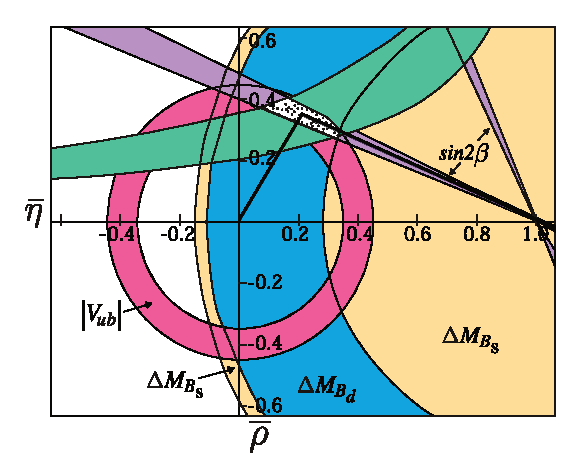
\includegraphics[width=\linewidth]{ckm04}
  \end{minipage}
\end{tabular}

\vspace{0.5 cm}
{\color{black} Complementary with $f_D$: see Topher Cawlfield's talk}

\end{slide}

\begin{slide}[Method]

Determine $\Upsilon \to e^+e^-$ decay rate by measuring $e^+e^- \to \Upsilon$ cross-section

{\Huge
\[ \Gamma_{ee} = \frac{{M_\Upsilon}^2}{6 \pi^2} \int \sigma(e^+e^- \to \Upsilon) \, dE \]
}

\vspace{0.5 cm}
\begin{center}
\begin{tabular}{p{0.5\linewidth} p{0.5 cm} p{0.4\linewidth}}
\begin{minipage}{\linewidth}
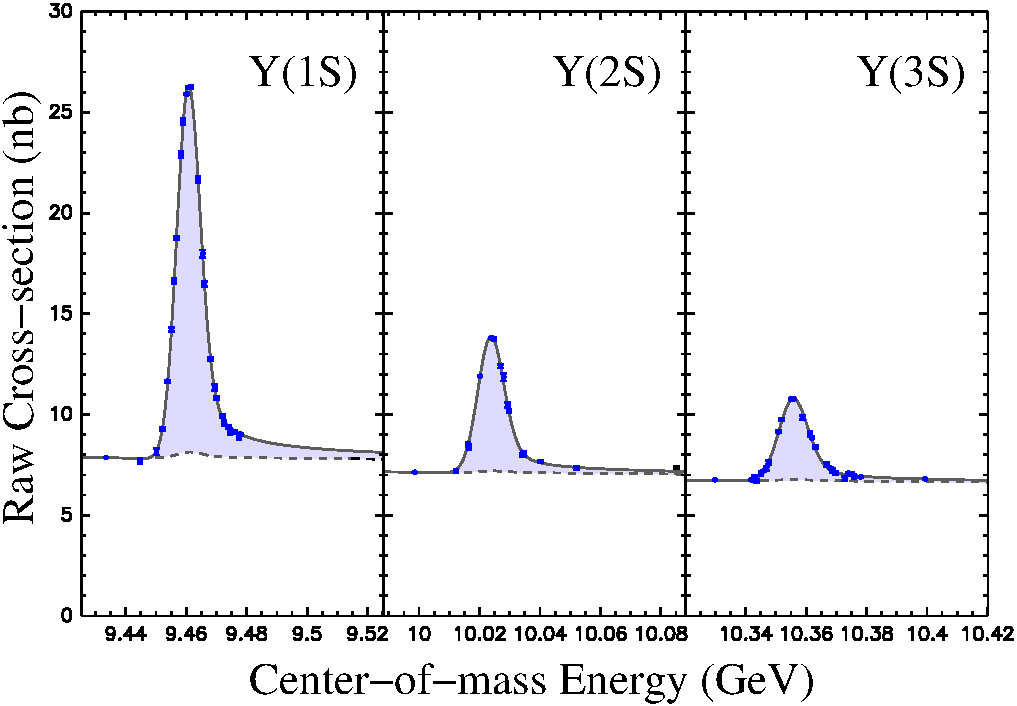
\includegraphics[width=\linewidth]{samplescans}
\end{minipage} & &
\begin{minipage}{\linewidth}
\begin{center}
Cornell Electron Storage Ring

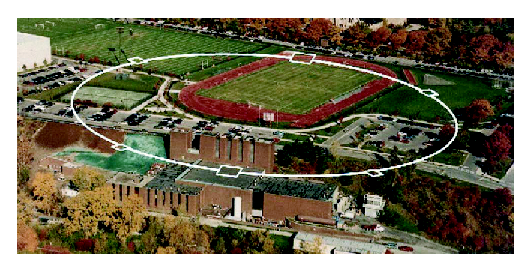
\includegraphics[width=0.8\linewidth]{aerial}

\vspace{0.5 cm}
\Large Integrated Luminosity (on+off peak)

\begin{tabular}{l l l}
  \us & 0.27+0.19 fb\inv & 4.9 million \\
  \uss & 0.08+0.41 fb\inv & 0.5 million \\
  \usss & 0.22+0.14 fb\inv & 0.9 million \\
\end{tabular}
\end{center}
\end{minipage}
\end{tabular}
\end{center}

\vspace{0.5 cm}
Measure $\sigma(e^+e^- \to \Upsilon \to \mbox{hadrons})$ at several beam energies

\vspace{0.5 cm}
Integrate spectrum without initial-state radiation convolution

\end{slide}

\begin{slide}[Backgrounds]

\vspace{1 cm}
\begin{center}
  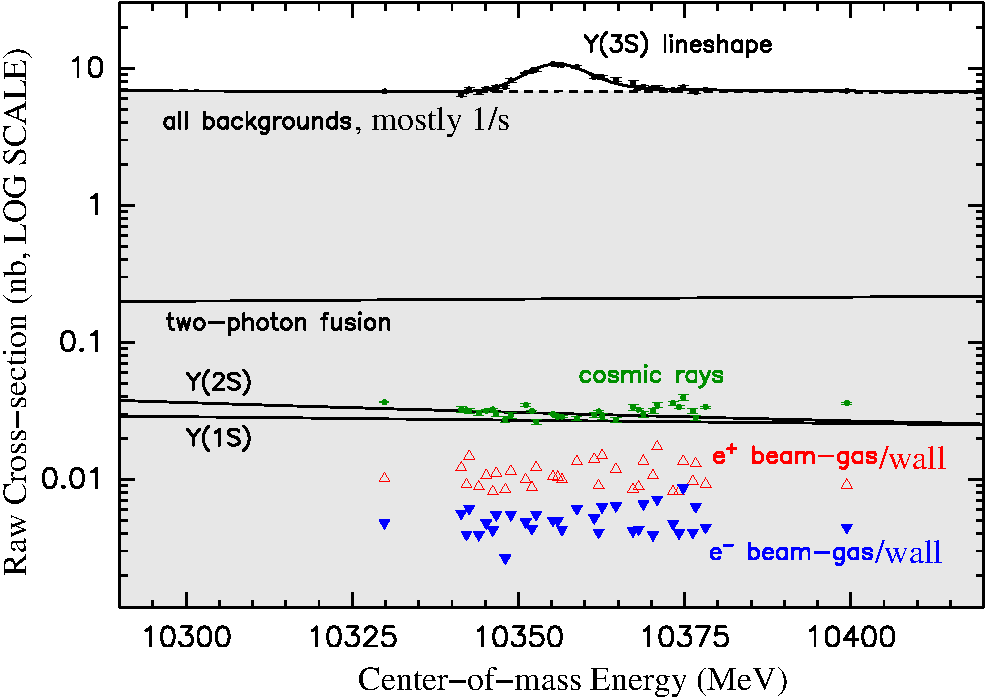
\includegraphics[width=0.9\linewidth, trim=0.5cm 2cm 0.5cm 2cm]{backgrounds}
\end{center}

\end{slide}

\begin{slide}[Efficiency]

\begin{tabular}{p{0.62\linewidth} c p{0.35\linewidth}}
  \begin{minipage}{\linewidth}
    \begin{itemize}\setlength{\itemsep}{0.75 cm}

      \item Select \mbox{$\Upsilon(2S) \to \pi^+ \pi^- \ \Upsilon(1S)$} by $\pi^+ \pi^-$ recoil mass

	\begin{center}
	  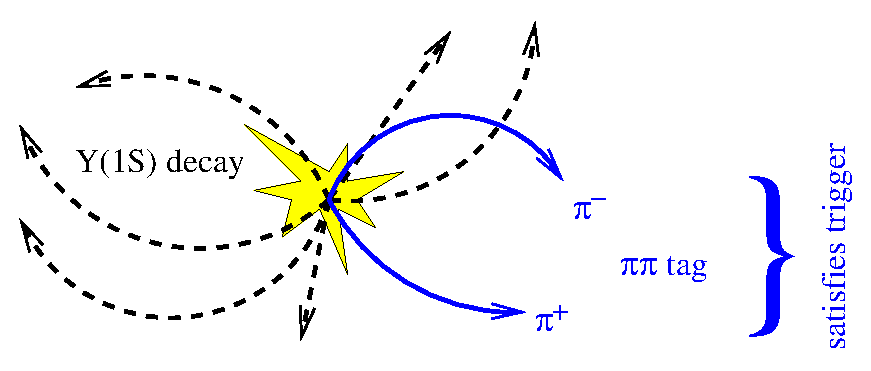
\includegraphics[width=0.9\linewidth]{twotoone}
	\end{center}

      \item Set of $\Upsilon(1S)$ events is unbiased, includes all decays

    \end{itemize}
  \end{minipage} & & \begin{minipage}{\linewidth}
    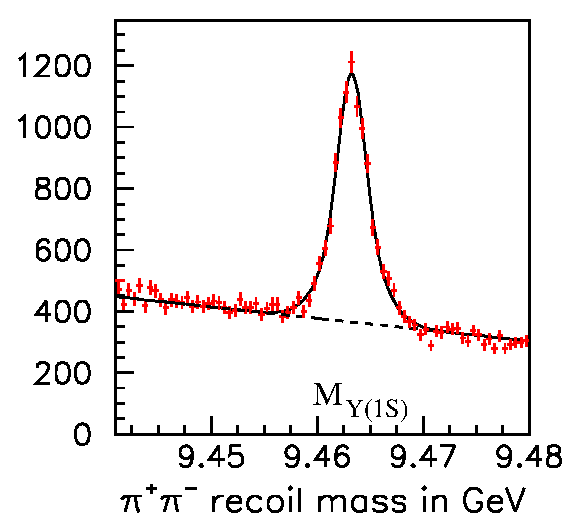
\includegraphics[width=\linewidth]{pipimass}
  \end{minipage}
\end{tabular}

\vspace{1 cm}
\begin{itemize}\setlength{\itemsep}{1.5 cm}

  \item \us\ efficiency = \#pass/\#total = (97.8 $\pm$ 0.5)\%

  \item For \uss\ and \usss\ efficiency, we extrapolate using Monte Carlo

\end{itemize}

\end{slide}

\begin{slide}[Integrated Luminosity]

\begin{itemize}

  \item Count $e^+e^- \to e^+e^-$ events and compare with theoretical cross-section

  \item Check overall scale with $e^+e^- \to \mu^+\mu^-$ and $e^+e^- \to \gamma\gamma$

\end{itemize}

\vspace{0.5 cm}
\begin{center}
  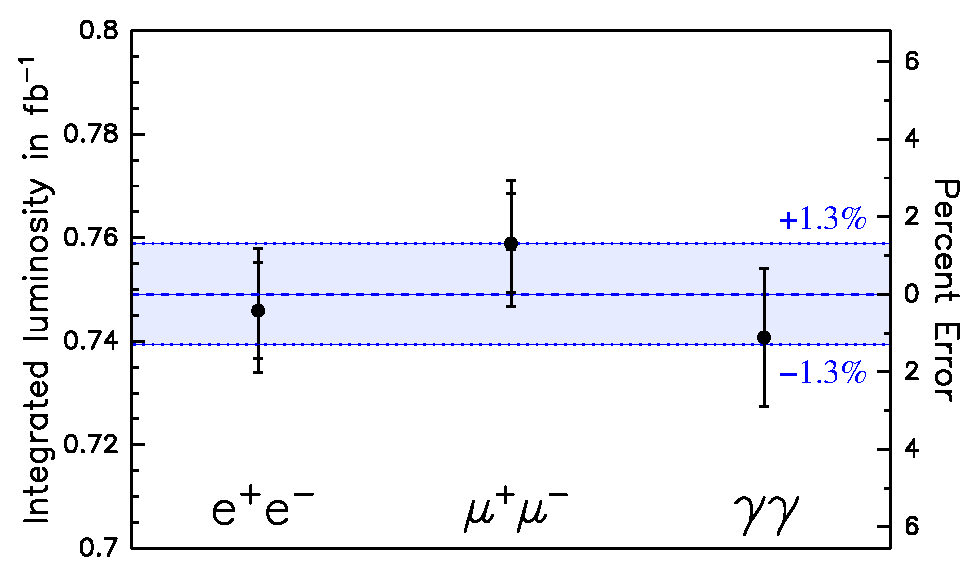
\includegraphics[width=0.85\linewidth]{luminosity}
\end{center}

\end{slide}

\begin{slide}[Beam Energy Uncertainty]

\begin{tabular}{p{0.6\linewidth} p{0.38\linewidth}}
  \begin{minipage}{\linewidth}
    \begin{minipage}{0.9\linewidth}
      \begin{itemize}\setlength{\itemsep}{0.75 cm}

	\item Beam energy determined by dipole magnet measurement

	\item Calibration drifts with time (0.5~MeV/month)

	\item Each resonance completely scanned in 48 hours (repeated
	scans for statistical precision)

        \item Measurements alternated above and below resonance peak

        \item Point of high slope repeated ({\color{red} 1 \& 5}):
        convert cross-section reproducibility into beam energy reproducibility

	\item $\Rightarrow$ 0.07~MeV uncertainty in center-of-mass differences, 0.2\% in \gee

	\end{itemize}
    \end{minipage}

  \end{minipage} &
  \begin{minipage}{\linewidth}
    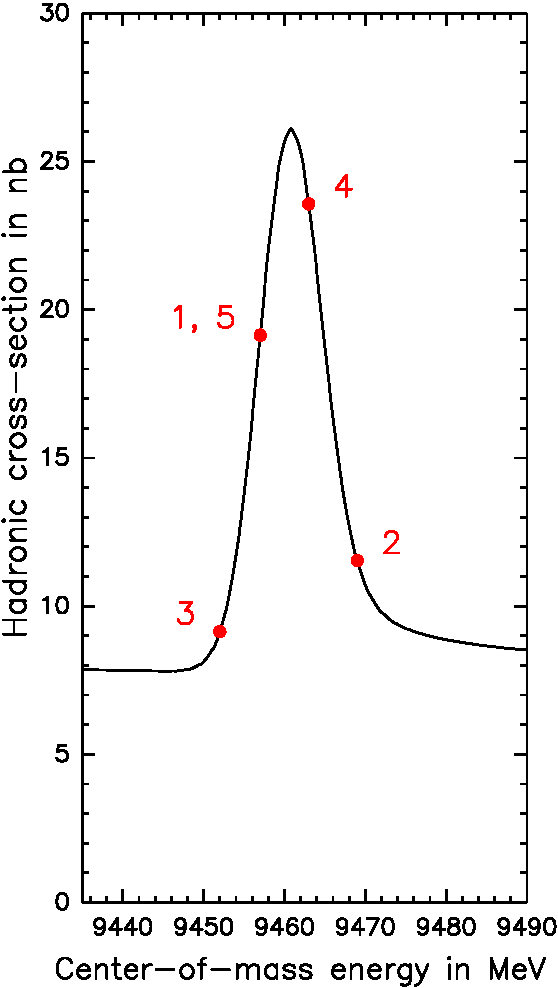
\includegraphics[width=\linewidth]{fitorder}
  \end{minipage}
\end{tabular}

\end{slide}

\begin{slide}[Fit Results]
\begin{center}

{\Large \boldmath
\hspace{0.5 cm} \begin{tabular}{c c c}
  $\chi^2/N_\subs{dof} = 1.3$ \mbox{\hspace{4.2 cm}} & $\chi^2/N_\subs{dof} = 1.6$ & \mbox{\hspace{4.2 cm}} $\chi^2/N_\subs{dof} = 1.0$
\end{tabular}}
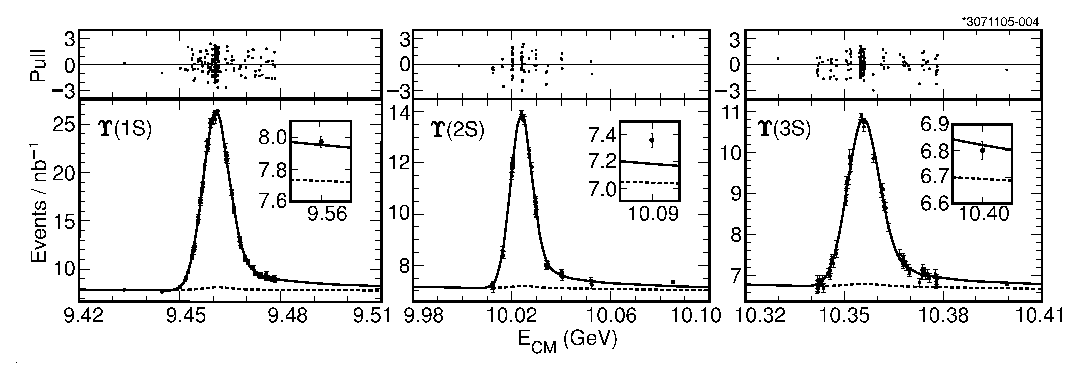
\includegraphics[width=\linewidth]{fits}

\vspace{1.2 cm}
\renewcommand{\arraystretch}{1.2}
\begin{tabular}{c c c c c}
  & & & Statistical & Systematic \\
  \boldmath $\Gamma_{ee}(1S)$ & \mbox{\hspace{0.25 cm}} = \mbox{\hspace{0.25 cm}} & 1.354 $\pm$ 0.004 $\pm$ 0.020 keV & 0.3\% & 1.5\% \\
  & & & \\
  \boldmath $\Gamma_{ee}(2S)$ & = & 0.619 $\pm$ 0.004 $\pm$ 0.010 keV & 0.7\% & 1.6\% \\
  & & & \\
  \boldmath $\Gamma_{ee}(3S)$ & = & 0.446 $\pm$ $\underbrace{\mbox{0.004}}_{\mbox{stat}}$ $\pm$ $\underbrace{\mbox{0.007}}_{\mbox{syst}}$ keV & 1.0\% & 1.5\%
\end{tabular}

\end{center}
\end{slide}

\begin{slide}[Interference with Continuum Hadrons]

Interference between $e^+e^- \to \Upsilon \to q\bar{q}$ and $e^+e^- \to q\bar{q}$ matters

\vfill
Phase difference cycles through resonance: destructive interference below resonance, \mbox{constructive} above

\vfill
Our fit prefers \qqbar-interference over no-interference by 3.7 standard deviations

\vfill
\begin{center}
\begin{tabular}{p{0.45\linewidth} p{0.45\linewidth}}
\begin{minipage}{\linewidth}
\vspace{1.5 cm}
{\color{red} red:} no interference

{\color{blue} blue:} exaggerated interference

\vspace{0.25 cm}
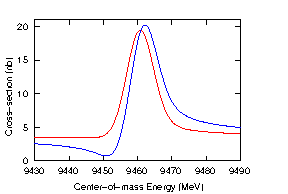
\includegraphics[width=\linewidth]{interference}
\end{minipage} &
\begin{minipage}{\linewidth}
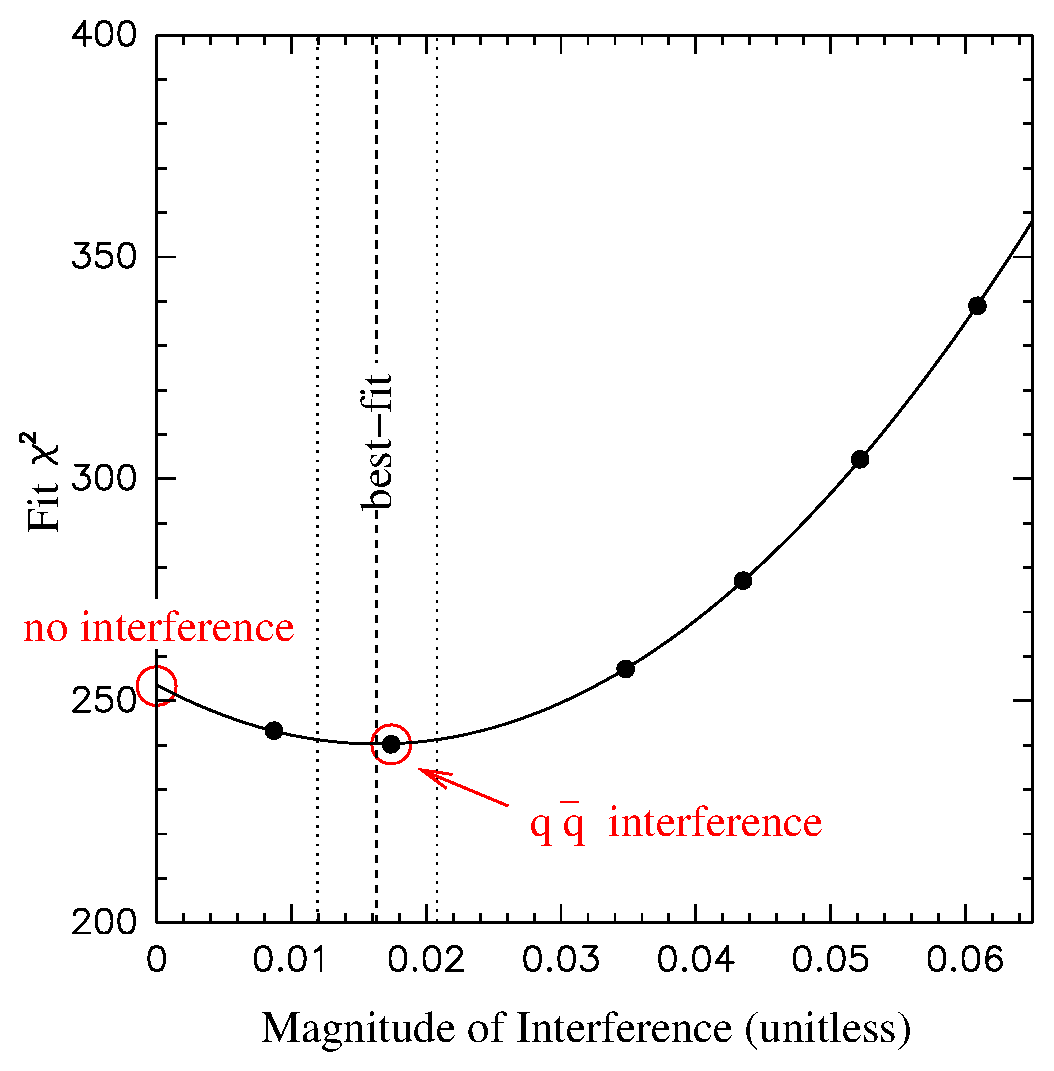
\includegraphics[width=\linewidth]{simpleintfit}
\end{minipage}
\end{tabular}
\end{center}

\end{slide}

\begin{slide}[Summary of Uncertainties]

\vspace{-1.6 cm}
\mbox{ } \hfill {\color{blue} $^*$Common to all resonances}

\vspace{1.6 cm}
\begin{center}
  \renewcommand{\arraystretch}{1.5}
  \begin{tabular}{l c c c}
    \hline\hline Contribution to \gee & \hspace{0.5 cm}\us\hspace{0.5 cm} & \hspace{0.5 cm}\uss\hspace{0.5 cm} & \hspace{0.5 cm}\usss\hspace{0.5 cm} \\\hline
    Correction for leptonic modes        	   & 0.2\%  & 0.2\%  & 0.3\%  \\
    {\color{blue} Hadronic efficiency$^*$} & {\color{blue} 0.5\%}  & {\color{blue} 0.5\%}  & {\color{blue} 0.5\%}  \\
    $Xe^+e^-$, $X\mu^+\mu^-$ correction  	   & 0      & 0.15\% & 0.13\% \\
    {\color{blue} Overall luminosity scale$^*$} & {\color{blue} 1.3\%}  & {\color{blue} 1.3\%}  & {\color{blue} 1.3\%}  \\
    Bhabha/$\gamma\gamma$ inconsistency  	   & 0.4\%  & 0.4\%  & 0.4\%  \\
    Beam energy measurement drift \hspace{0.5 cm}  & 0.2\%  & 0.2\%  & 0.2\%  \\
    Fit function shape                   	   & 0.1\%  & 0.1\%  & 0.1\%  \\
    $\chi^2$ inconsistency               	   & 0.2\%  & 0.6\%  & 0      \\\hline
    Total systematic uncertainty         	   & {\color{red} 1.5\%}  & {\color{red} 1.6\%}  & {\color{red} 1.5\%}  \\
    Statistical uncertainty              	   & 0.3\%  & 0.7\%  & 1.0\%  \\\hline
    Total                                	   & {\color{red} 1.5\%}  & {\color{red} 1.8\%}  & {\color{red} 1.8\%}  \\\hline\hline
  \end{tabular}
\end{center}

\end{slide}

\begin{slide}[Results!]

\begin{center}
\renewcommand{\arraystretch}{1.8}
\begin{tabular}{c c c c}
%%   \boldmath $\Gamma_{ee}\Gamma_\subs{had}/\Gamma_\subs{tot}(1S)$ & \mbox{\hspace{0.25 cm}} = \mbox{\hspace{0.25 cm}} & 1.252 $\pm$ 0.004 $\pm$ 0.019 keV & \mbox{\hspace{0.5 cm}} 1.6\% \mbox{\hspace{0.5 cm}}  \\
%%   \boldmath $\Gamma_{ee}\Gamma_\subs{had}/\Gamma_\subs{tot}(2S)$ & = & 0.581 $\pm$ 0.004 $\pm$ 0.009 keV & 1.7\% \\
%%   \boldmath $\Gamma_{ee}\Gamma_\subs{had}/\Gamma_\subs{tot}(3S)$ & = & 0.413 $\pm$ 0.004 $\pm$ 0.006 keV & 1.7\% \\\hline

  \boldmath $\Gamma_{ee}(1S)$ & \mbox{\hspace{0.25 cm}} = \mbox{\hspace{0.25 cm}} & 1.354 $\pm$ 0.004 $\pm$ 0.020 keV & \mbox{\hspace{0.5 cm}} 1.5\% \mbox{\hspace{0.5 cm}} \\
  \boldmath $\Gamma_{ee}(2S)$ & = & 0.619 $\pm$ 0.004 $\pm$ 0.010 keV & 1.8\% \\
  \boldmath $\Gamma_{ee}(3S)$ & = & 0.446 $\pm$ 0.004 $\pm$ 0.007 keV & 1.8\% \\\hline

  \boldmath $\Gamma_{ee}(2S)/\Gamma_{ee}(1S)$ & = & 0.457 $\pm$ 0.004 $\pm$ 0.004 keV & 1.2\% \\
  \boldmath $\Gamma_{ee}(3S)/\Gamma_{ee}(1S)$ & = & 0.329 $\pm$ 0.003 $\pm$ 0.003 keV & 1.3\% \\
  \boldmath $\Gamma_{ee}(3S)/\Gamma_{ee}(2S)$ & = & 0.720 $\pm$ 0.009 $\pm$ 0.007 keV & 1.6\% \\\hline

  \boldmath $\Gamma(1S)$ & = & 54.4 $\pm$ 0.2 $\pm$ 0.8 $\pm$ 1.6 keV & 3.3\% \\
  \boldmath $\Gamma(2S)$ & = & 30.5 $\pm$ 0.2 $\pm$ 0.5 $\pm$ 1.3 keV & 4.6\% \\
  \boldmath $\Gamma(3S)$ & = & 18.6 $\pm$ 0.2 $\pm$ 0.3 $\pm$ $\underbrace{\mbox{0.9}}_{{\mathcal B}_{\mu\mu}}$ keV & 5.2\% \\

\end{tabular}
\end{center}

\vspace{0.5 cm}
{\Large \hfill \renewcommand{\arraystretch}{1.5} \begin{tabular}{l l}
\gee: & hep-ex/0512056, to be published in Phys.\ Rev.\ Lett.\ (March 2006) \\
\bmm: & G.S.~Adams {\it et al.} (CLEO Collaboration), Phys.\ Rev.\ Lett.\  {\bf 94}, 012001 (2005)
\end{tabular}}

\end{slide}

\begin{slide}[History]

\begin{center}
  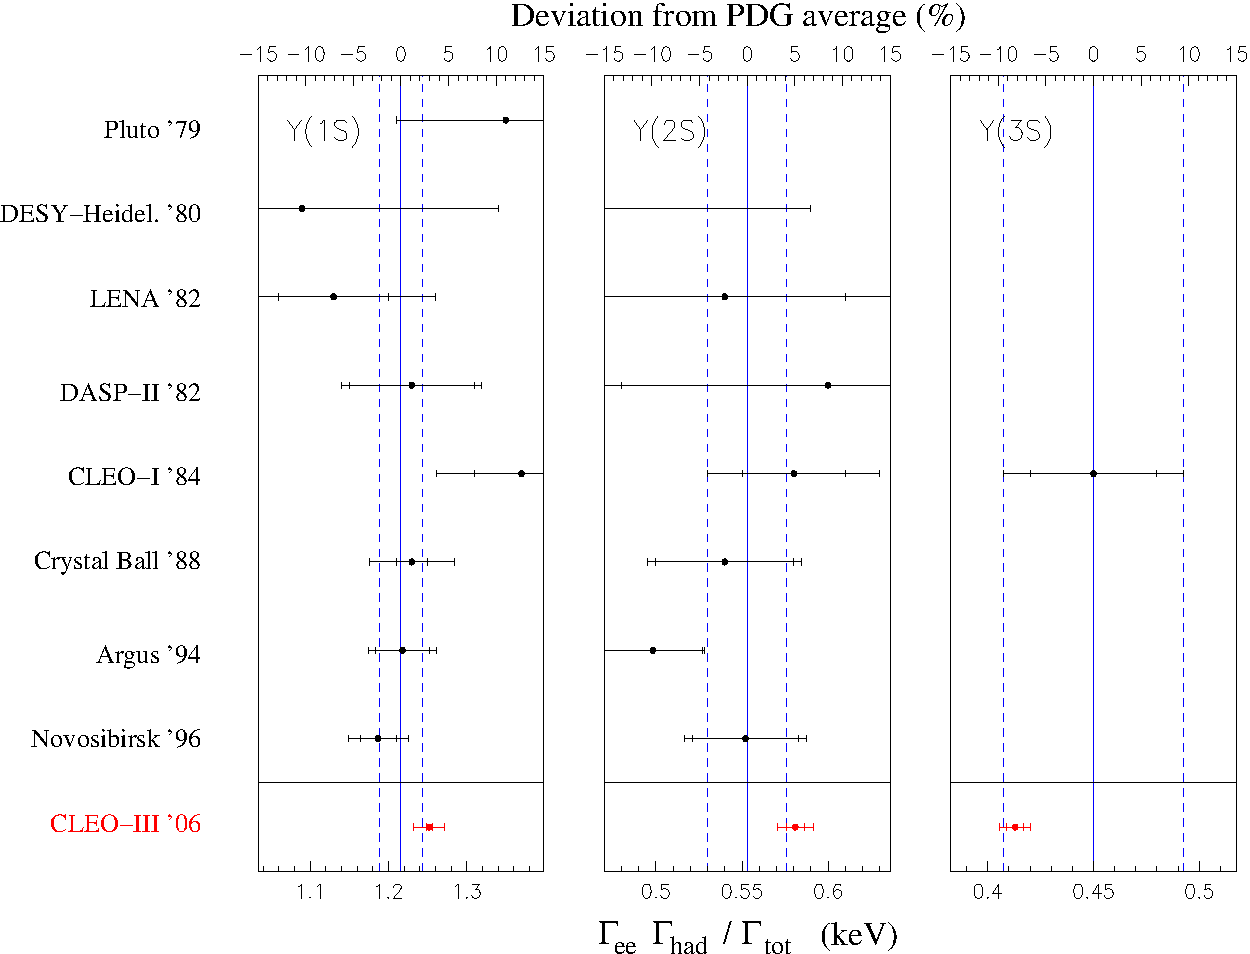
\includegraphics[width=0.9\linewidth]{historyplot}
\end{center}

\end{slide}

\begin{slide}[Comparison with Lattice QCD]

\begin{itemize}

  \item Lattice QCD results are preliminary

  \item Final results will have few percent precision in $\Gamma_{ee}(nS)/\Gamma_{ee}(mS)$ and $\sim$10\% in $\Gamma_{ee}(nS)$

\end{itemize}

\vspace{0.5 cm}
\begin{center}
  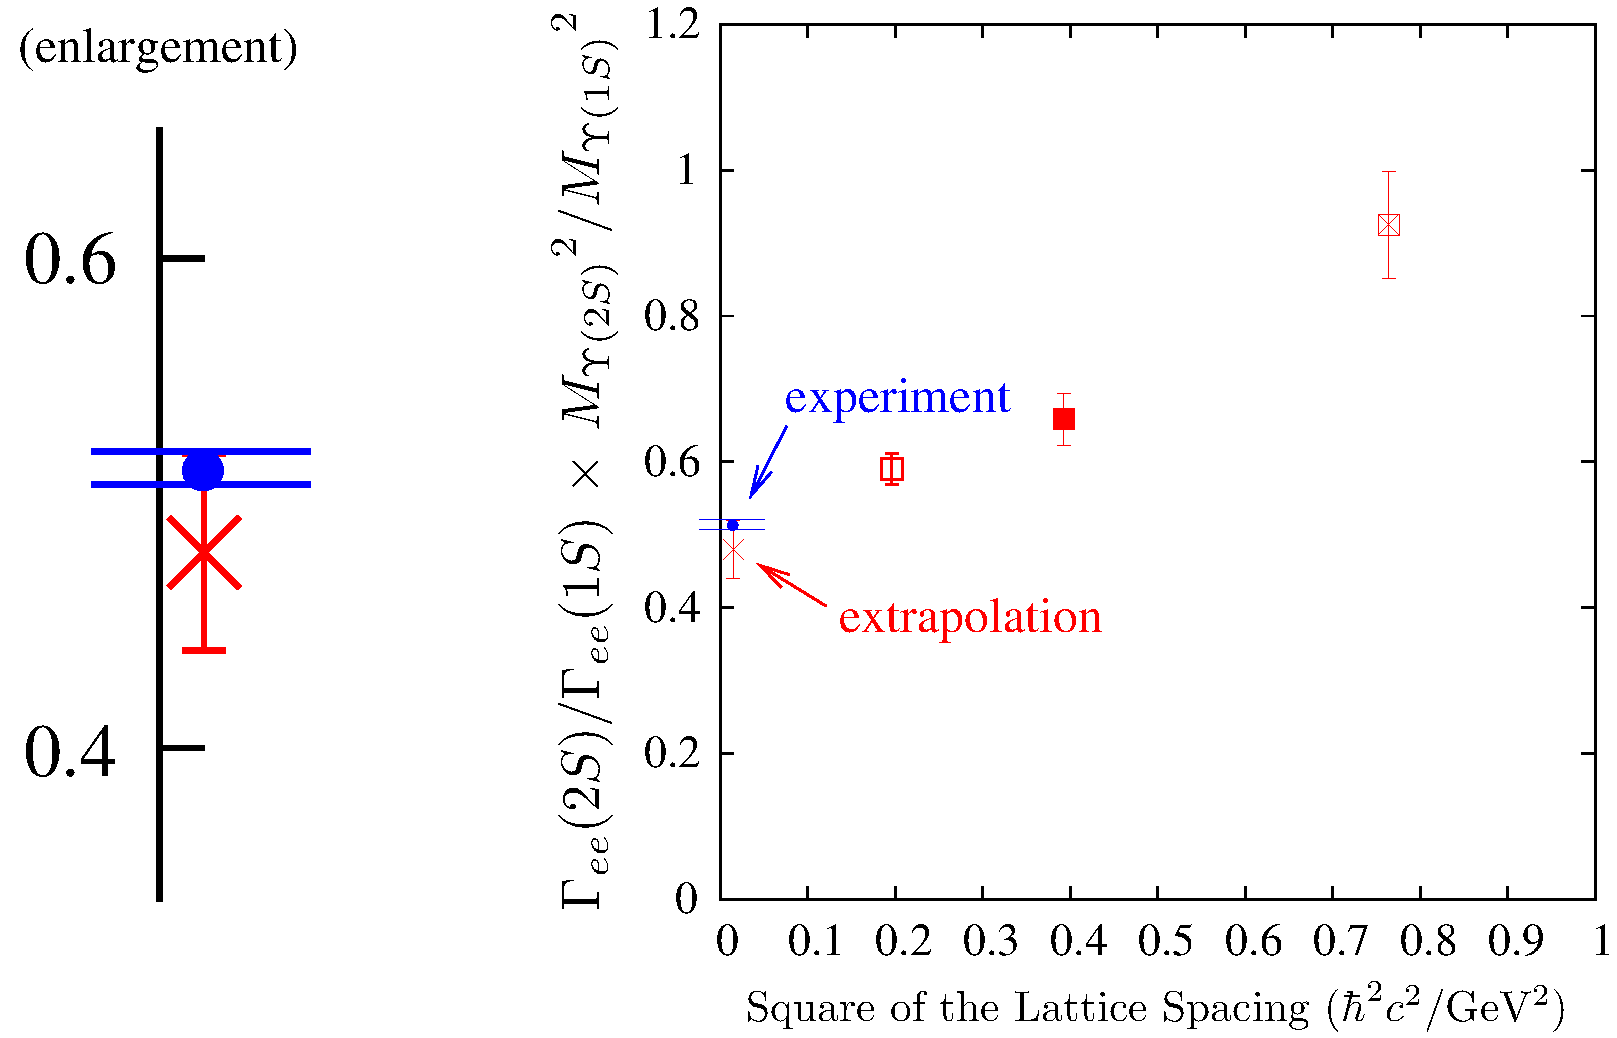
\includegraphics[width=0.75\linewidth]{latticespacingagain}
\end{center}

\Large
\vspace{0.5 cm}
\renewcommand{\arraystretch}{1.2}
\begin{tabular}{l l}
  Lattice QCD & A.~Gray {\it et al.} [HPQCD Collaboration], Phys.\ Rev.\ D {\bf 72}, 094507 (2005) \\
  Experiment & hep-ex/0512056, to be published in Phys.\ Rev.\ Lett.\ (March 2006) \\
             & and J.\ Pivarski, Cornell University, Ph.D. thesis
\end{tabular}

\end{slide}

\end{document}
